%
%   Prof. Dr. Julian Reichwald
%   auf Basis einer Vorlage von Prof. Dr. Jörg Baumgart
%   DHBW Mannheim
%
%
%	ACHTUNG: Für das Erstellen des Literaturverzeichnisses wird das modernere Paket biblatex
%			 in Kombination mit biber verwendet -- nicht mehr das ältere BibTex!
% 			 Bitte stellen Sie ggf. Ihre TeX-Umgebung
% 			 entsprechend ein (z.B. TeXStudio: Einstellungen --> Erzeugen --> Standard Bibliographieprogramm: biber)
%

\documentclass[
	12pt,
	BCOR=5mm,
	DIV=10,
	headinclude=on,	
	footinclude=off,
	parskip=half,
	bibliography=totoc,
	listof=entryprefix,
	toc=listof,
	pointlessnumbers
	]{scrreprt}

%	Konfigurationsdatei einziehen
% !TEX root =  master.tex

%		LANGUAGE SETTINGS AND FONT ENCODING 
%
\usepackage[ngerman]{babel} 	% German language
\usepackage[utf8]{inputenc}
\usepackage[german=quotes]{csquotes} 	% correct quotes using \enquote{}
\usepackage[T1]{fontenc}



%\usepackage[english]{babel}   % For english language
%\usepackage{csquotes} 	% Richtiges Setzen der Anführungszeichen mit \enquote{}

% 		HYPERREF
%
\usepackage[
	hidelinks=true % keine roten Markierungen bei Links
]{hyperref}

% Zwei eigene Befehle zum Setzen von Autor und Titel. Ausserdem werden die PDF-Informationen richtig gesetzt.
\newcommand{\TitelDerArbeit}[1]{\def\DerTitelDerArbeit{#1}\hypersetup{pdftitle={#1}}}
\newcommand{\AutorDerArbeit}[1]{\def\DerAutorDerArbeit{#1}\hypersetup{pdfauthor={#1}}}
\newcommand{\Firma}[1]{\def\DerNameDerFirma{#1}}
\newcommand{\Kurs}[1]{\def\DieKursbezeichnung{#1}}


% Correct superscripts 
\usepackage{fnpct}




%		CALCULATIONS
%
\usepackage{calc} % Used for extra space below footsepline



%		BIBLIOGRAPHY SETTINGS
%

% Uncomment the next three lines for author-year-style with footnotes (Chicago)
%\usepackage[backend=biber, autocite=footnote, style=authoryear, dashed=false]{biblatex} 	%Use Author-Year-Cites with footnotes


% Uncomment the next line for IEEE-style 
\usepackage[backend=biber, autocite=inline, style=ieee]{biblatex} 	% Use IEEE-Style (e.g. [1])

% Uncomment the next line for alphabetic style 
% \usepackage[backend=biber, autocite=inline, style=alphabetic]{biblatex} 	% Use alphabetic style (e.g. [TGK12])

% Uncomment the next two lines vor Harvard-Style 
%\usepackage[backend=biber, style=apa]{biblatex} 	
%\DeclareLanguageMapping{german}{german-apa}


\DefineBibliographyStrings{ngerman}{  %Change u.a. to et al. (german only!)
	andothers = {{et\,al\adddot}},
}

%%% Uncomment the following lines to support hard URL breaks in bibliography 
%\apptocmd{\UrlBreaks}{\do\f\do\m}{}{}
%\setcounter{biburllcpenalty}{9000}% Kleinbuchstaben
%\setcounter{biburlucpenalty}{9000}% Großbuchstaben


\setlength{\bibparsep}{\parskip}		%add some space between biblatex entries in the bibliography
\addbibresource{bibliography.bib}	%Add file bibliography.bib as biblatex resource


%		FOOTNOTES 
%
% Count footnotes over chapters
\usepackage{chngcntr}
\counterwithout{footnote}{chapter}

%	ACRONYMS
%%%
%%% WICHTIG: Installieren Sie das neueste Acronyms-Paket!!!
%%%
\makeatletter
\usepackage[printonlyused]{acronym}
\@ifpackagelater{acronym}{2015/03/20}
  {%
    \renewcommand*{\aclabelfont}[1]{\textbf{\textsf{\acsfont{#1}}}}
  }%
  {%
  }%
\makeatother

%		LISTINGS
\usepackage{listings}	%Format Listings properly
\renewcommand{\lstlistingname}{Quelltext} 
\renewcommand{\lstlistlistingname}{Quelltextverzeichnis}
\lstset{numbers=left,
	numberstyle=\tiny,
	captionpos=b,
	basicstyle=\ttfamily\small}


%		EXTRA PACKAGES
\usepackage{lipsum}    %Blindtext
\usepackage{graphicx} % use various graphics formats
\usepackage[german]{varioref} 	% nicer references \vref
\usepackage{caption}	%better Captions
\usepackage{booktabs} %nicer Tabs
\usepackage{array}
\usepackage{longtable}
%\newcolumntype{P}[1]{>{\raggedright\arraybackslash}p{#1}}


%		ALGORITHMS
\usepackage{algorithm}
\usepackage{algpseudocode}
\renewcommand{\listalgorithmname}{Algorithmenverzeichnis }
\floatname{algorithm}{Algorithmus}


%		FONT SELECTION: Entweder Latin Modern oder Times / Helvetica
\usepackage{lmodern} %Latin modern font
%\usepackage{mathptmx}  %Helvetica / Times New Roman fonts (2 lines)
%\usepackage[scaled=.92]{helvet} %Helvetica / Times New Roman fonts (2 lines)

%		PAGE HEADER / FOOTER
%	    Warning: There are some redefinitions throughout the master.tex-file!  DON'T CHANGE THESE REDEFINITIONS!
\RequirePackage[automark,headsepline,footsepline]{scrlayer-scrpage}
\pagestyle{scrheadings}
\renewcommand*{\pnumfont}{\upshape\sffamily}
\renewcommand*{\headfont}{\upshape\sffamily}
\renewcommand*{\footfont}{\upshape\sffamily}
\renewcommand{\chaptermarkformat}{}
\RedeclareSectionCommand[beforeskip=0pt]{chapter}
\clearscrheadfoot

\ifoot[\rule{0pt}{\ht\strutbox+\dp\strutbox}DHBW Mannheim]{\rule{0pt}{\ht\strutbox+\dp\strutbox}DHBW Mannheim}
\ofoot[\rule{0pt}{\ht\strutbox+\dp\strutbox}\pagemark]{\rule{0pt}{\ht\strutbox+\dp\strutbox}\pagemark}

\ohead{\headmark}

\usepackage{xcolor}
\usepackage{multirow}
\usepackage{tabularx}
\usepackage{pgf-pie} 

\begin{document}

\TitelDerArbeit{Pentesting Project X}
\AutorDerArbeit{Luka Tsipitsoudis}
\Kurs{TINF20CS1}

\begin{titlepage}
    \begin{minipage}{\textwidth}
            \vspace{-2cm}
            \noindent
            %  
\includegraphics[scale=0.71]{img/firmenlogo.jpg} 
             \hfill   
             
\includegraphics{img/logo.jpg}
    \end{minipage}
    \vspace{1em}
    \sffamily
    \begin{center}
        \textsf{\large{}Duale Hochschule Baden-W\"urttemberg\\[1.5mm] Mannheim}\\[2em]
        \textsf{\textbf{\Large{}Pentest Report}}\\[3mm]
        \textsf{\textbf{\DerTitelDerArbeit}} \\[1.5cm]
        \textsf{\textbf{\Large{}Studiengang Cyber Security}\\[3mm]}
        
        \vspace{3em}
    \vfill
    
    \begin{minipage}{\textwidth}
    
    \begin{tabbing}
        Wissenschaftlicher Betreuer: \hspace{0.85cm}\=\kill
        Verfasser: \> \DerAutorDerArbeit \\[1.5mm]
        Matrikelnummer: \> 4110112 \\[1.5mm]
        Kurs: \> \DieKursbezeichnung \\[1.5mm]
        % Bearbeitungszeitraum: \> 18.10.2022 -- 18.04.2023\\
        Abgabedatum: \> 18.04.2023\\ [1.5mm]
        Betreuer: \> Pr. Dr. Johannes Bauer\\
        % Ausbildungsfirma: \> \DerNameDerFirma  \\[1.5mm]
        % Betrieblicher Betreuer: \> Oliver Grimm \\
    \end{tabbing}
    
    \vspace{2cm}
    Unterschrift:  \> \_\_\_\_\_\_\_\_\_\_\_\_\_\_\_\_\_\_ 
    \end{minipage}
    
    \end{center}
    
    \end{titlepage}

\pagenumbering{roman} % Römische Seitennummerierung
\normalfont

%--------------------------------
% Verzeichnisse - nicht benötige Verzeichnisse bitte auskommentieren / löschen.
%--------------------------------

% Ehrenwörtliche Erklärung ewerkl.tex einziehen
% % !TEX root =  master.tex

\clearpage
\chapter*{Ehrenwörtliche Erklärung}

% Wird die folgende Zeile auskommentiert, erscheint die ehrenwörtliche
% Erklärung im Inhaltsverzeichnis.

% \addcontentsline{toc}{chapter}{Ehrenwörtliche Erklärung}
Ich versichere hiermit, dass ich meine Projektarbeit mit dem Thema: \textit{\DerTitelDerArbeit} selbstständig verfasst und keine anderen als die angegebenen Quellen und Hilfsmittel benutzt habe. Ich versichere zudem, dass die eingereichte elektronische Fassung mit der gedruckten Fassung übereinstimmt.

\vspace{3cm}
Mannheim, dd.mm.yyy

\textbf{Ort, Datum} \hfill Luka Tsipitsoudis


%   Sperrvermerk
% \chapter*{Sperrvermerk}
Der Inhalt dieser Arbeit: 

\textit{\glqq Entwicklung  einer Software zur Entscheidung der richtigen Projekt Methode. Welche Projektmethode passt zu meinem Projekt? \grqq{}}

darf weder als Ganzes noch in Auszügen Personen außerhalb des Prüfungsprozesses und des Evaluationsverfahrens zugänglich gemacht werden, sofern keine anders lautende Genehmigung des Dualen Partners vorliegt. 

[Ende der Sperrfrist: unbegrenzt]

\vspace{3cm}
Mannheim, 29.08.2022

\textbf{Ort, Datum} \hfill \DerAutorDerArbeit

\cleardoublepage



%	Kurzfassung
%\chapter*{Abstract}

\textbf{Deutsche Version} 

\clearpage
\textbf{Englische Version}





%	Inhaltsverzeichnis
\tableofcontents

%	Abbildungsverzeichnis
\listoffigures

%	Tabellenverzeichnis
%\listoftables

%	Listingsverzeichnis
%\lstlistoflistings

% 	Algorithmenverzeichnis
%\listofalgorithms

% 	Abkürzungsverzeichnis (siehe Datei acronyms.tex!)
\clearpage
\chapter*{Abkürzungsverzeichnis}	
\addcontentsline{toc}{chapter}{Abkürzungsverzeichnis}


\begin{acronym}[RDBMS]
	\acro{DUT}{Device Under Testing}
\end{acronym}

\ohead{Acronyms} % Neue Header-Definition


%--------------------------------
% Start des Textteils der Arbeit
%--------------------------------
\clearpage
\ihead{\chaptername~\thechapter} % Neue Header-Definition (inner header)
\ohead{\headmark} % Neue Header-Definition (outer header)
\pagenumbering{arabic}  % Arabische Seitenzahlen

\chapter{Introduction}

\section{Scope}
This Penetration Test Report is based on the E-Mail from our client Pr. Dr. Bauer. The E-Mail was send on 2023-02-20 13:56 with the subject ”Schriftliche Beschreibung der Laborarbeit 'Offensive Security'” (SHA-224 sum: \newline  dafaf185c6d7ec66804121fd25b8f1165f96aea3e183efbb660d250d). The given scenario is a black box test.
The given \ac{DUT} is a Raspberry Pi.
The \ac{DUT} might be interacting with external systems. Those systems are not included in the scope of this test.
The \ac{DUT} is running on a ”Cortex-A53” CPU which is based on an aarch64 ARM architecture (whole CPU information can be found in the appendix). The running OS is Debian with a 5.15.61-v8+ kernel (whole kernel information can be found in the appendix).



\newpage
\section{Severities}
Each finding in this report is assigned a severity level. The following table defines the severity levels used in this report. Some findings may be estimated different in the organizational context.

\begin{table}[H]
    \centering
    \label{tab:severity}
    \begin{tabular}{|c|p{10cm}|}
    \hline
    \multicolumn{1}{|c|}{\textbf{Severity Level}} & \multicolumn{1}{c|}{\textbf{Definition}} \\ \hline
    \textcolor{green!50!blue}{\textbf{Low}} & Vulnerability that has a limited impact on the system or data and may not require immediate attention. It represents a low risk to the organization and can be addressed in a routine patching cycle or by implementing a simple configuration change.\\ \hline
    \textcolor{orange}{\textbf{Medium}} & Vulnerability that has a moderate impact on the system or data and requires some effort to exploit. It represents a moderate risk to the organization and may require a more thorough analysis and remediation effort. \\ \hline
    \textcolor{red}{\textbf{High}} & Vulnerability that has a significant impact on the system or data and can be easily exploited. It represents a high risk to the organization and requires immediate attention and remediation. \\ \hline
    \end{tabular}
    \caption{Severity Levels}
\end{table}
    
    
    

\section{Classification}
Each finding in this report is assigned to a classification. The following table defines the classification levels used in this report. Notice that some findings could be assigned to multiple classifications. For a better overview in this report every finding is assigned only to one classification.

\begin{table}[H]
    \centering
    \label{tab:classification}
    \begin{tabular}{|c|p{10cm}|}
    \hline
    \multicolumn{1}{|c|}{\textbf{Classification}} & \multicolumn{1}{c|}{\textbf{Definition}} \\ \hline
    \textbf{Information Disclosure} & Information disclosure vulnerabilities are those that allow an attacker to obtain sensitive information from the system.\\ \hline
    \textbf{Denial of Service} & Denial of service vulnerabilities are those that allow an attacker to prevent the system from providing its services.\\ \hline
    \textbf{Elevation of Privilege} & Elevation of privilege vulnerabilities are those that allow an attacker to gain access to resources that are normally protected from the user.\\ \hline
    \textbf{Misonfiguration} & Vulnerabilities that are caused by configurations and can lead to an exploit. \\ \hline
    \end{tabular}
    \caption{Classification}
    \end{table}
\section{Effort to Fix}
Each finding in this report is assigned to an effort to fix level. The following table defines the effort to fix levels used in this report. Notice that this is only a recommendation. Some findings may be estimated different in the organizational context.

\begin{table}[H]
    \centering
    \label{tab:effort}
    \begin{tabular}{|c|p{10cm}|}
    \hline
    \multicolumn{1}{|c|}{\textbf{Effort to Fix Level}} & \multicolumn{1}{c|}{\textbf{Definition}} \\ \hline
    \textcolor{green!50!blue}{\textbf{Low}} & The vulnerability can be fixed with a simple configuration change or a routine patching cycle.\\ \hline
    \textcolor{orange}{\textbf{Medium}} & The vulnerability can be fixed with a moderate effort for example with a different or new implementation.\\ \hline
    \textcolor{red}{\textbf{High}} & The vulnerability can be fixed with a high effort like an architectural change.\\ \hline
    \end{tabular}
    \caption{Effort to Fix}
\end{table}

\chapter{Management Summary}
Short Summary for non technical people.
what are key takeeaways and recommendations?
how urgent is acting neccessary?
\chapter{Technical Summary}

summery for technical people

\section{Findings Overview}
The following table contains all findings sorted by severity:


\begin{table}[H]
  \centering
  \label{tab:example}
  \begin{tabularx}{\textwidth}{|X|X|X|X|}
    \hline
    \textbf{Finding} & \textbf{Classification} & \textbf{Severity} & \textbf{Effort to Fix} \\
    \hline

    Weak password for User Bluey & Weak Password & \textcolor{red}{\textbf{High}} & \textcolor{green!50!blue}{\textbf{Low}}\\
    \hline
    No Brute-Force Protection for
SSH & Misconfiguration & \textcolor{red}{\textbf{High}} & \textcolor{green!50!blue}{\textbf{Low}}\\
    \hline
    Root Read Access via Port 443 & Vulnerable Software & \textcolor{red}{\textbf{High}} & \textcolor{green!50!blue}{\textbf{Low}}\\
    \hline
    No Encryption for Webserver on
    Port 80 & Misconfiguration & \textcolor{red}{\textbf{High}} & \textcolor{green!50!blue}{\textbf{Low}}\\
    \hline
    Sudo Access on Less for User
    bluey & Misconfiguration & \textcolor{red}{\textbf{High}} & \textcolor{green!50!blue}{\textbf{Low}}\\
    \hline
    Path Traversal on Apache Server & Information Disclosure & \textcolor{red}{\textbf{High}} & \textcolor{orange}{\textbf{Medium}}\\
    \hline
    Webserver allows vulnerable
Protocols & Misconfiguration & \textcolor{red}{\textbf{High}} & \textcolor{orange}{\textbf{Medium}}\\
    \hline
    Privilige Escalation via SSH & Misconfiguration & \textcolor{red}{\textbf{High}} & \textcolor{orange}{\textbf{Medium}}\\
    \hline
    Weak Cipher Suites for
Webserver on Port 443 & Misconfiguration & \textcolor{red}{\textbf{High}} & \textcolor{orange}{\textbf{Medium}}\\
    \hline
  \end{tabularx}
  \caption{Findings}
\end{table}


\begin{table}[H]
    \centering
    \label{tab:2}
    \begin{tabularx}{\textwidth}{|X|X|X|X|}
        \hline
        \textbf{Finding} & \textbf{Classification} & \textbf{Severity} & \textbf{Effort to Fix} \\
        \hline

    Vulnerable Software leads to
Remote Code Execution
& Vulnerable Software & \textcolor{red}{\textbf{High}} & \textcolor{orange}{\textbf{Medium}}\\
\hline
Vulnerable Management Server
on Port 20321 & Vulnerable Software & \textcolor{red}{\textbf{High}} & \textcolor{orange}{\textbf{Medium}}\\
\hline
SD-Card not encrypted & Misconfiguration & \textcolor{red}{\textbf{High}} & \textcolor{orange}{\textbf{Medium}}\\
\hline
\end{tabularx}
\end{table}


\section{Used Tools}
\chapter{Findings}
\chapter{Finding 1}

\section{Finding Beschreibung}
\textbf{Klassifikation:}
\newline \textbf{Severity:}

\section{Finding Auswirkung}

\section{Finding Lösung}

\section{Finding Quellen}

\clearpage
\section{Finding 2 - Vulnerable OpenSSH Version}
%center under chapter title a one row table with 6 coloumns and no borders
\begin{center}
\begin{tabular}{c c c c}
    \textbf{Classification:} & Vulnerable Software Version & \textbf{Severity: \textcolor{orange}{Medium}} &  \\ \textbf{CVE:} & CVE-2021-28041, CVE-2021-41617 &\\
\end{tabular}
\end{center}


\subsection{Finding Description}
The \ac{DUT} is running a vulnerable OpenSSH version (8.4p1). This version is vulnerable to the following CVEs: CVE-2021-28041, CVE-2021-41617.

\subsection{Finding Impact}
Following exploits can be used to gain access to the \ac{DUT}:
\newline
\newline
\textbf{CVE-2021-28041:} This vulnerability enables an attacker to carry out unauthorized code execution on a target system remotely. The vulnerability stems from an error in the ssh-agent, where a remote attacker can lure the victim to connect to a server where the attacker has root access.
\newline
\newline
\textbf{CVE-2021-41617:} When OpenSSH is used with non default configurations privilige escalation is possible. (Check configuration)

\subsection{Evaluation of Results}
\begin{center}
    \begin{tabular}{cccc}
    \textbf{Effort to Fix:} & &\ \textbf{\textcolor{green!50!blue}{Low}}\
    \end{tabular}
\end{center}
Update OpenSSH to 9.2/9.2p1 (Check). This can be done by running the following command:
\begin{lstlisting}[language=bash]
$ sudo apt update
$ sudo apt install openssh-server
\end{lstlisting}


\section{Finding 4 - Vulnerable Apache Version}
%center under chapter title a one row table with 6 coloumns and no borders
\vspace*{-0,3cm}
\begin{center}
    \begin{tabular}{c c c c}
        \textbf{Classification:} & Vulnerable Software Version & \textbf{Severity:} & \textbf{\textcolor{orange}{Medium}}  
        \end{tabular}
\end{center}

%make spacing on top of the table less
\vspace*{-0,8cm}
\begin{center}
    \begin{tabular}{c c}
        \textbf{CVE:} & CVE-2023-25690, CVE-2023-27522, CVE-2006-20001, \\ & CVE-2022-36760, CVE-2022-37436
    \end{tabular}
\end{center}

On port 80 the \ac{DUT} is running a vulnerable Apache version (\textbf{”Apache 2.4.54”}). This version has multiple vulnerabilities and shouldn't be used in production. \newline
The following vulnerabilities are known from \ac{CVE} but haven't been exploited on the \ac{DUT}.


\subsection{Finding Impact}
\textbf{CVE-2023-25690:} When the mod\_proxy configuration is enabled a HHTP smuggling attack is possible, which could bypass the access controls.
\newline\newline
\textbf{CVE-2023-27522:} This vulnerability allows an attacker to send a origin header which contains special characters to the server. This could be used truncate/split the response forwarded to the client.
\newline\newline
\textbf{CVE-2006-20001:} This vulnerability allows an attacker to send a specific if request to the server, which could be used to crash the process.
\newline\newline
\textbf{CVE-2022-36760:} Due to an incosistent interpretation of HTTP requests of the server it could be possible for attackers to smuggle HTTP requests to the \ac{AJP} server. 
\newline\newline
\textbf{CVE-2022-37436:} A malicious backend has the ability to terminate the response headers prematurely, leading to certain headers being integrated into the response body. Following headers which serve a security function, they will not be comprehended by the client.

\subsection{Finding Cause}

\subsection{Finding Details}

\subsection{Evaluation of Results}
\begin{center}
    \begin{tabular}{cccc}
    \textbf{Effort to Fix:} & &\ \textbf{\textcolor{orange}{Medium}}\
    \end{tabular}
\end{center}
How do you judge the individual technical findings (severity, likelihood)?
What is your suggested remediation, if there is one?
How can the customer validate their remediation is effective once implemented?
\section{Finding 4 - Vulnerable Apache Version}
%center under chapter title a one row table with 6 coloumns and no borders
\vspace*{-0,3cm}
\begin{center}
    \begin{tabular}{c c c c}
        \textbf{Classification:} & Vulnerable Software Version & \textbf{Severity:} & \textbf{\textcolor{orange}{Medium}}  
        \end{tabular}
\end{center}

%make spacing on top of the table less
\vspace*{-0,8cm}
\begin{center}
    \begin{tabular}{c c}
        \textbf{CVE:} & CVE-2023-25690, CVE-2023-27522, CVE-2006-20001, \\ & CVE-2022-36760, CVE-2022-37436
    \end{tabular}
\end{center}

On port 80 the \ac{DUT} is running a vulnerable Apache version (\textbf{”Apache 2.4.54”}). This version has multiple vulnerabilities and shouldn't be used in production. \newline
The following vulnerabilities are known from \ac{CVE} but haven't been exploited on the \ac{DUT}. Some of these vulnerabilities may only be exploitable with specific configurations. Nevertheless, all of these vulnerabilities are shown to provide transparency and to show the possible impact of the vulnerabilities.


\subsection{Finding Impact}
\textbf{CVE-2023-25690:} When the mod\_proxy configuration is enabled a HHTP smuggling attack is possible, which could bypass the access controls.
\newline\newline
\textbf{CVE-2023-27522:} This vulnerability allows an attacker to send a origin header which contains special characters to the server. This could be used truncate/split the response forwarded to the client.
\newline\newline
\textbf{CVE-2006-20001:} This vulnerability allows an attacker to send a specific if request to the server, which could be used to crash the process.
\newline\newline
\textbf{CVE-2022-36760:} Due to an incosistent interpretation of HTTP requests of the server it could be possible for attackers to smuggle HTTP requests to the \ac{AJP} server. 
\newline\newline
\textbf{CVE-2022-37436:} A malicious backend has the ability to terminate the response headers prematurely, leading to certain headers being integrated into the response body. Following headers which serve a security function, they will not be comprehended by the client.

\subsection{Finding Details}
%add code snippet
\begin{lstlisting}[language=bash]
$ nmap -A 172.16.0.29

Starting Nmap 7.93 ( https: //nmap.org ) at 2023-03-06 09:30 CET
Nmap scan report for 172.16.0.29
Host is up (0.00051s latency).

PORT STATE SERVICE VERSION
80/tcp open http Apache httpd 2.4.54 ((Debian))
\end{lstlisting}

\subsection{Evaluation of Results}
\begin{center}
    \begin{tabular}{cccc}
    \textbf{Effort to Fix:} & &\ \textbf{\textcolor{green!50!blue}{Low}}\
    \end{tabular}
\end{center}
To fix this vulnerability the Apache Server has to be updated to a newer version. This could be done with the following command:
\begin{lstlisting}[language=bash]
$ apt update && apt install apache2
\end{lstlisting}

\section{Finding 5 - Path Traversal on Apache Server}
%center under chapter title a one row table with 6 coloumns and no borders
\vspace*{-0,3cm}
\begin{center}
    \begin{tabular}{c c c c}
        \textbf{Classification:} & Information Disclosure & \textbf{Severity:} & \textbf{\textcolor{red}{High}}  
        \end{tabular}
\end{center}

\vspace*{-0,8cm}
\begin{center}
    \begin{tabular}{c c}
        \textbf{CVE:} &
    \end{tabular}
\end{center}

On the Apache Server of the \ac{DUT} (port 80) it is possible to access directories via path traversal. By adding the path ”/home/...” to the URL it is possible to see directories which seem to be users of the \ac{DUT}.
The directories are empty.

\subsection{Finding Impact}
The Impact of this finding is an severe Information Disclosure. Attackers could try to guess passwords for the found users and eventually gain access to the \ac{DUT}.

\subsection{Finding Details}
A way to find the path is to use a nmap scan with the ”http-enum” script:
\begin{lstlisting}[language=bash]
$ nmap -A --script -http-enum 172.16.0.29

PORT STATE SERVICE VERSION
80/top open http Apache httpd 2.4.54 ((Debian))
|_http-server-header: Apache/2.4.54 (Debian)
| http-enum:
|_ /home/:
Potentially interesting directory w/ listing on 
'apache/2.4.54 (debian)'
\end{lstlisting}


To see the directory it is possible to visit the URL in a web browser:
%insert an image but in this subsection
\begin{figure}[h]
    \centering
    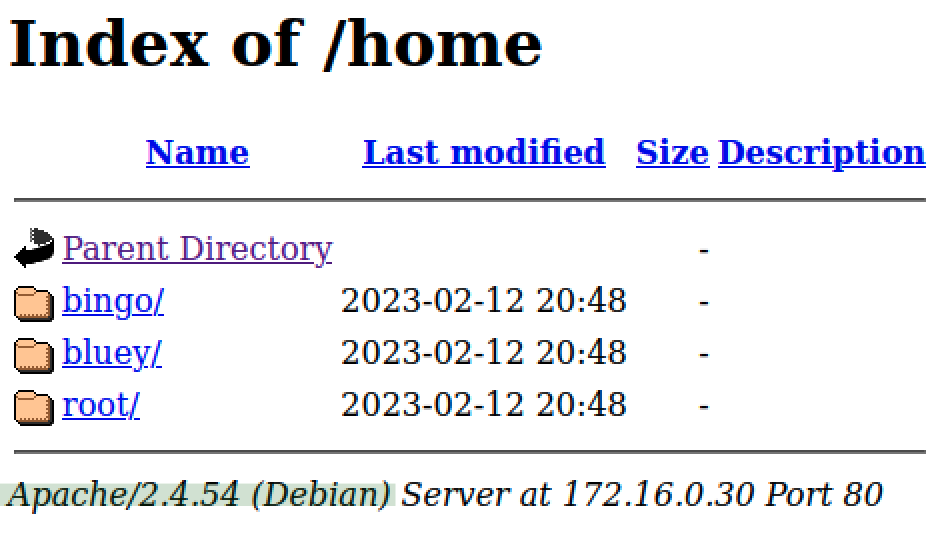
\includegraphics[width=0.8\textwidth]{img/apache-version.png}
    \caption{Path Traversal}
    \label{fig:fin5}
\end{figure}

\subsection{Evaluation of Results}
\begin{center}
    \begin{tabular}{cccc}
    \textbf{Effort to Fix:} & &\ \textbf{\textcolor{orange}{Medium}}\
    \end{tabular}
\end{center}
The Server should validate the path before accessing it. A possible solution could be to whitelist the allowed paths, which should be accessible. This would prevent accessing directories of the \ac{DUT} which are not intended to be accessed by the user.
\section{Finding 6 - Weak password for User Bluey}
%center under chapter title a one row table with 6 coloumns and no borders
\vspace*{-0,3cm}
\begin{center}
    \begin{tabular}{c c c c}
        \textbf{Classification:} & Weak Password & \textbf{Severity:} & \textbf{\textcolor{red}{High}}  
        \end{tabular}
\end{center}

\vspace*{-0,7cm}
\begin{center}
    \begin{tabular}{c c}
        \textbf{CVE:} & CVE-2022-1039
    \end{tabular}
\end{center}

Using the Tool ”Hydra” the Password for the User ”bluey” was found in a very short amount of time with Brute Force. The Password is ”phoenix”. As a passwordlist the file ”rockyou.txt” was used which contains about 14 million common passwords. This file can be found online and is accessible for everyone.

\subsection*{Finding Impact}
With the password it is possible to login to the \ac{DUT} as the User ”bluey” via ssh. This allows attackers to gain access to the \ac{DUT} and to execute commands as the User ”bluey”. This could lead for example to a 
\ac{RCE} or to a privlige escaltion (horizontal or vertical).

\subsection*{Finding Details}
The Password was found using the Tool ”Hydra” with the following command:
\begin{lstlisting}[language=bash]
$ hydra -l bluey -P rockyou.txt 172.16.0.29 ssh -t 4 -V -I
\end{lstlisting}

After the password was found it was possible to login to the \ac{DUT} as the User ”bluey” via ssh:
%image here
\begin{figure}[h]
    \centering
    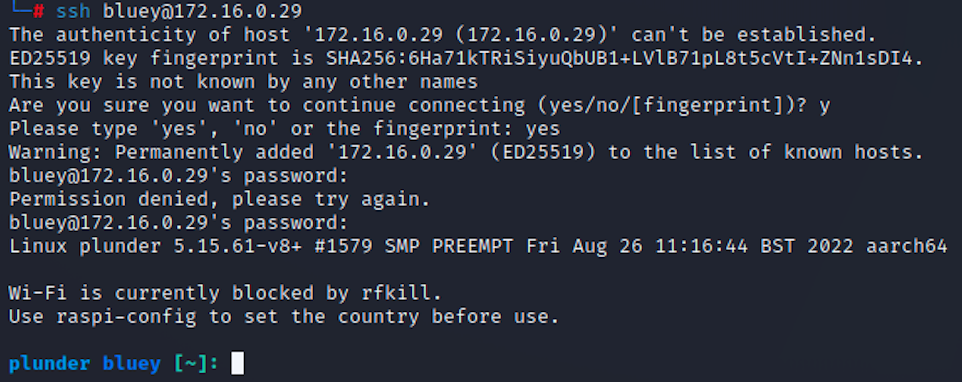
\includegraphics[width=0.8\textwidth]{img/ssh-access-bluey.png}
    \caption{Login as User Bluey}
    \label{fig:fin6}
\end{figure}


\subsection*{Evaluation of Results}
\begin{center}
    \begin{tabular}{cccc}
    \textbf{Effort to Fix:} & &\ \textbf{\textcolor{green!50!blue}{Low}}\
    \end{tabular}
\end{center}
The password should be changed immediately. Notice that passwordlength is the most important aspect. Don't use common passwords.

\section{Finding 7 - No Brute-Force Protection for SSH}

%center under chapter title a one row table with 6 coloumns and no borders
\vspace*{-0,3cm}
\begin{center}
    \begin{tabular}{c c c c}
        \textbf{Classification:} & Misconfiguration & \textbf{Severity:} & \textbf{\textcolor{orange}{Medium}}  
        \end{tabular}
\end{center}

\vspace*{-0,8cm}
\begin{center}
    \begin{tabular}{c c}
        \textbf{CVE:} & 
    \end{tabular}
\end{center}



\subsection{Finding Impact}


\subsection{Finding Details}

\subsection{Evaluation of Results}
\begin{center}
    \begin{tabular}{cccc}
    \textbf{Effort to Fix:} & &\ \textbf{\textcolor{green!50!blue}{Low}}\
    \end{tabular}
\end{center}


\clearpage
\pagenumbering{roman}
\setcounter{page}{9}
%	Literaturverzeichnis
\clearpage
\ihead{}
\printbibliography[title=Literaturverzeichnis]
\cleardoublepage

% Der Anhang beginnt hier - jedes Kapitel wird alphabetisch aufgezählt. (Anhang A, B usw.)
%\appendix
%\ihead{\appendixname~\thechapter} % Neue Header-Definition


% appendix.tex einziehen
%\chapter{Appendix}
Complete CPU information:
%image
\begin{figure}[H]
    \centering
    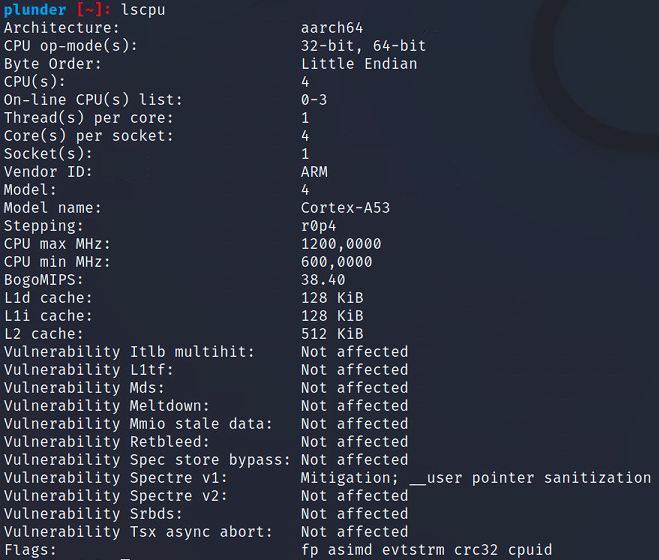
\includegraphics[width=1\textwidth]{img/prozessor_info.png}
    \caption{CPU Information}
    \label{fig:cpuinfo}
\end{figure}

Complete kernel information:
%image
\begin{figure}[H]
    \centering
    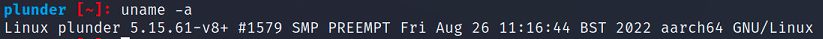
\includegraphics[width=1\textwidth]{img/uname-a.png}
    \caption{Kernel Information}
    \label{fig:kernelinfo}
\end{figure}

Decompiled ”check\_version.pyc”:
%image
\begin{figure}[H]
    \centering
    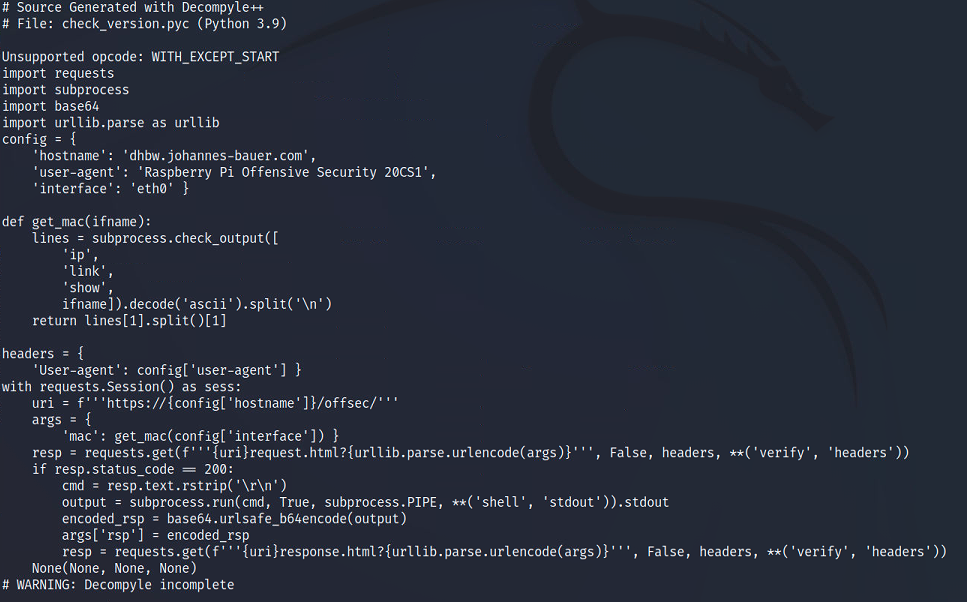
\includegraphics[width=1\textwidth]{img/check_version_decompiled.png}
    \caption{Decompiled check\_version.pyc}
    \label{fig:check_version}
\end{figure}

Decompiled ”fde\_setup.pyc”:
%image
\begin{figure}[H]
    \centering
    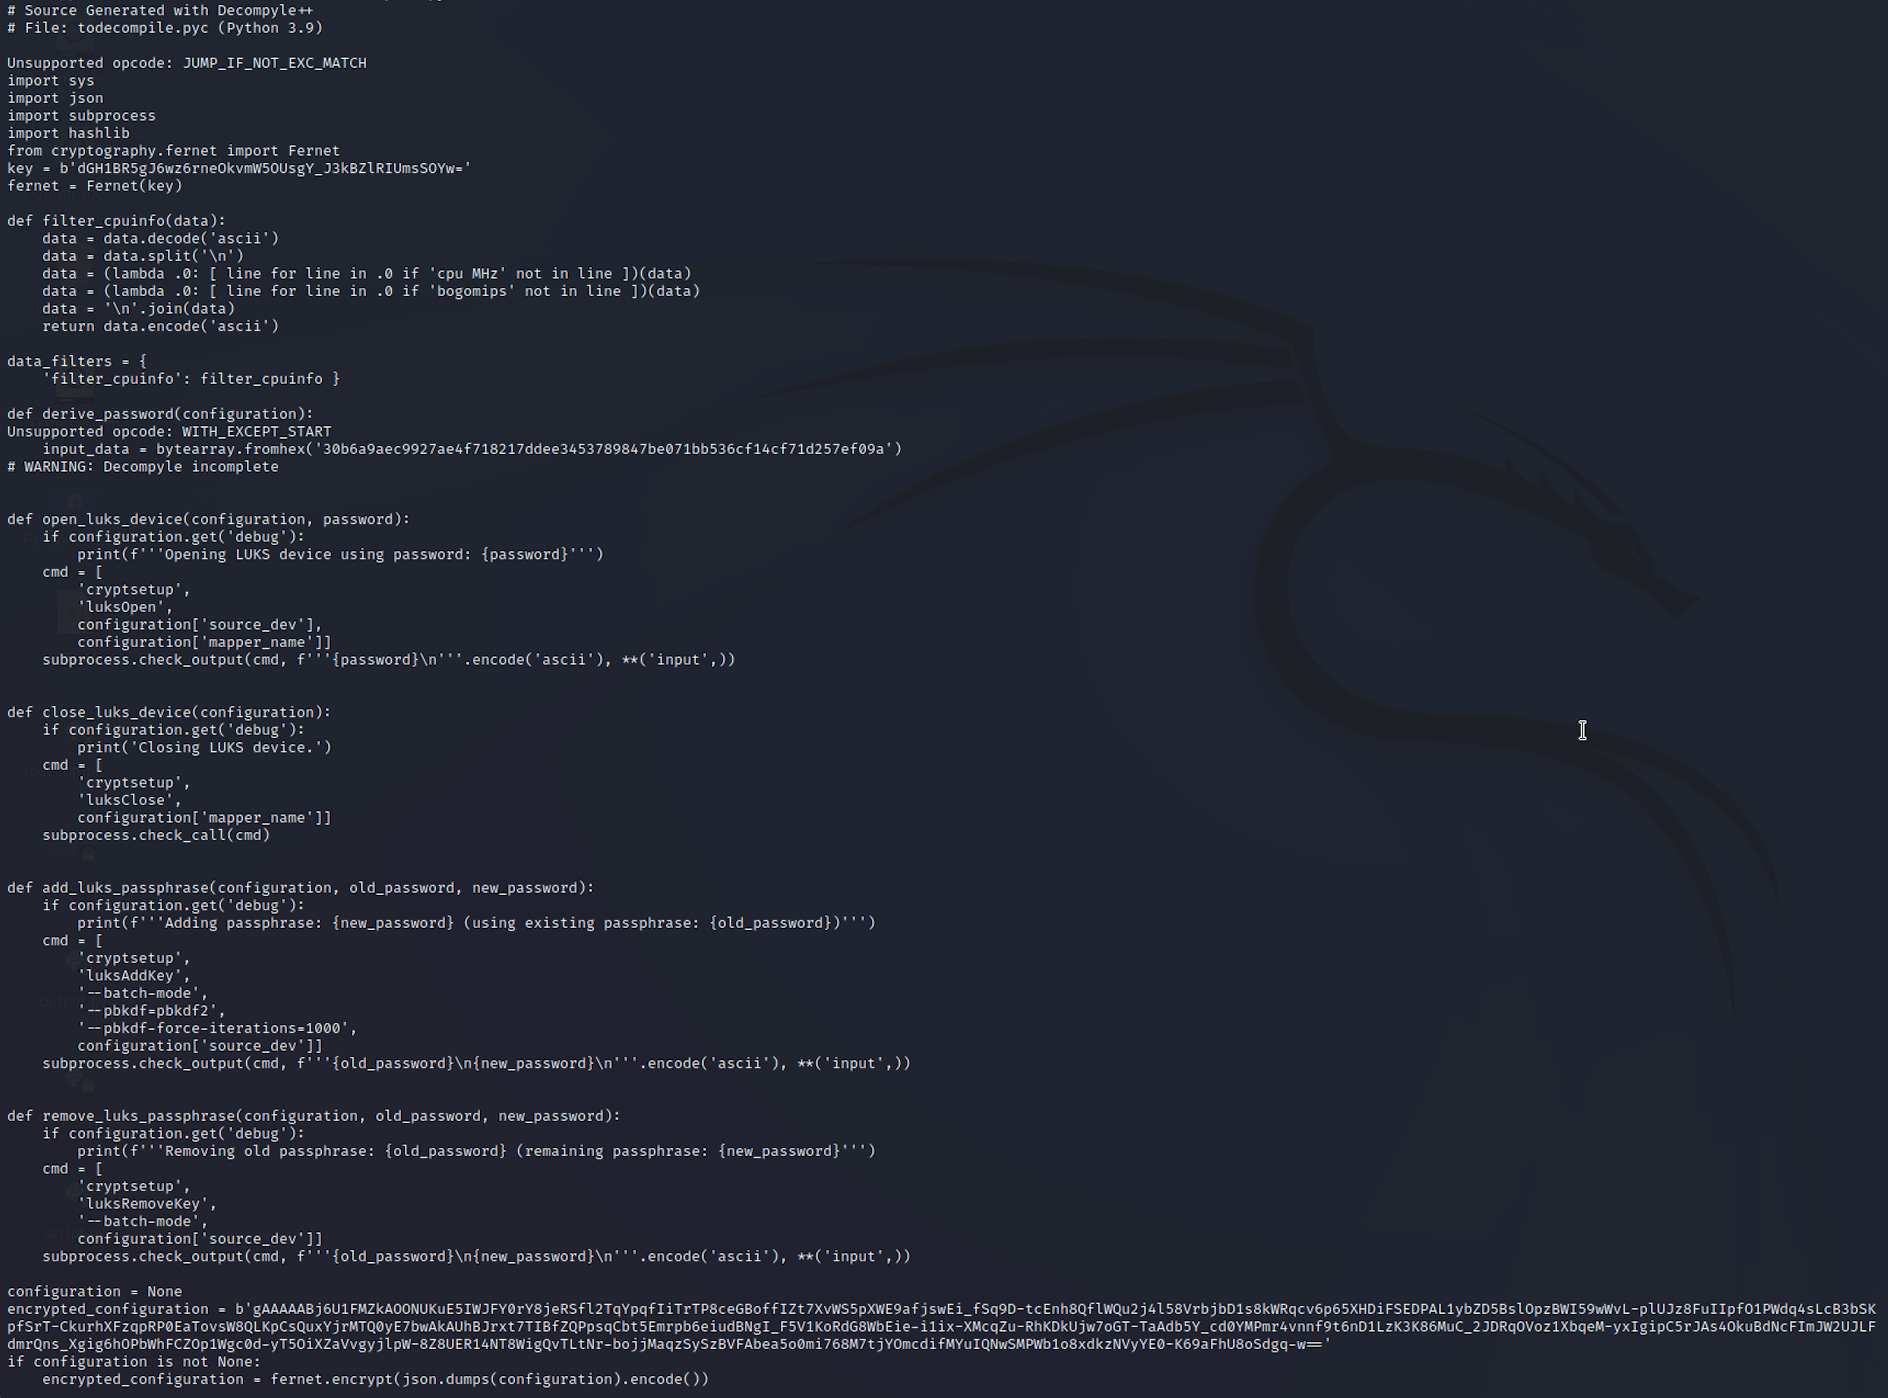
\includegraphics[width=1\textwidth]{img/dec_fde.png}
    \caption{Decompiled fde\_setup.pyc}
    \label{fig:fde_setup}
\end{figure}



\end{document}
